
\twocolumn[{%
\begin{center}
  {\LARGE \textbf{\textsf{Top Quark Seminar 7}}} \\
  \vspace{1em}
  {\Large \textbf{\textsf{Igor Babuschkin}}} \\
  \vspace{1em}
  {\large \textbf{\textsf{10th February 2015}}}
  \section*{Summary of \enquote{Search for top quark decays $t\to qH$ with $H\to\gamma\gamma$ using the ATLAS detector}}
\end{center}
}]

\noindent
The paper\cite{aad} documents a search for flavour-changing neutral currents in the decay of a top quark to an up-type quark and a Higgs boson performed using data taken at the ATLAS detector corresponding to integrated luminosities of \SI{4.7}{\text{fb}^{-1}} at $\sqrt{s} = \SI{7}{TeV}$ and \SI{20.3}{\text{fb}^{-1}} at $\sqrt{s} = \SI{8}{TeV}$.

Specifically, $t\overline{t}$ events were studied where one of the top quarks decays to $Wb$ and the $W$ decays either leptonically or hadronically (which are the dominant Standard Model processes) and the other top quark might decay through the previously mentioned flavour-changing neutral current involving the Higgs boson.

The analysis proceeded as follows:

The selection of the $H\to\gamma \gamma$ analysis, which consists of cuts on $E_T$ as well as identification and isolation requirements for the photons is used to select $H$ candidates.
In addition, several requirements are applied to select for a $t\overline{t}$ event.
These are chosen depending on whether the second top quark decay is supposed to have decayed hadronically or semi-leptonically.

In the case of a hadronic decay, this means selecting events with at least four jets of which at least one must be $b$-tagged.
If the invariant mass of one of the jets and the two photons, or the invariant mass of the other three jets is close to the top quark mass, the event is selected.
The authors state that they did not use $b$-tag association or a restriction on the reconstructed $m_W$ mass as selection criteria, as these didn't improve the sensitivity of the measurement.

For the semi-leptonic decay of the top quark, a cut on the transverse mass of the reconstructed $W$ boson is performed.

The presence of the theorized flavour changing neutral current would lead to a nonzero branching fraction for $t\to c(u) H$, and thus to an excess of Higgs bosons in the diphoton invariant mass beyond the Standard Model prediction.

To investigate the presence of such an excess, the authors evaluated a combined likelihood model for the diphoton mass distribution simultaneously over all data samples (hadronic/leptonic and \num{7}/\SI{8}{TeV}).
Higgs bosons produced by Standard Model processes constitute a background that peaks directly below the expected signal.
The cross section for Higgs boson production is thus constrained to a value calculated by combining the previous $ggF$, VBF, $WH$, $ZH$ and $t\overline{t}H$ measurements.
The results of the fit are displayed in figure \ref{mgammagamma}.

\begin{figure}
  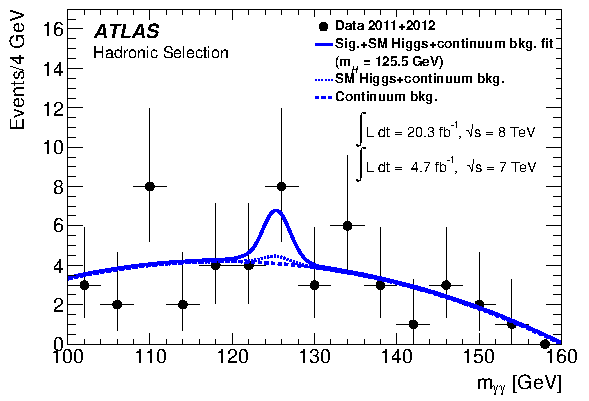
\includegraphics[width=0.5\textwidth]{figures/mgammagamma.pdf}
  \caption{Results of fit to the diphoton invariant mass.\cite{aad}}
  \label{mgammagamma}
\end{figure}

To account for nuisance parameters in the model, the Profile Likelihood method was chosen.
The fit then yields $3.1^{+4.3}_{-3.7}$ as the number of signal events.
An upper confidence limit of \SI{0.79}{\percent} on the $t\to q H$ branching fraction is then set using the $\text{CL}_\text{s}$ method.


